\chapter{Crittografia}

\section{Introduzione}

La crittografia è una scienza antichissima che consiste nel codificare e
decodificare l'informazione.
L'operazione di codifica permette di ottenere un testo codificato a partire da
un “testo in chiaro” che
può essere letto da tutti.
L'operazione di decodifica invece, consiste nel ricavare un testo in chiaro
partendo da un
testo cifrato. Ambedue le operazioni si basano su un algoritmo e sulla chiave;
l'algoritmo è
certamente pubblico. La sicurezza del sistema è data dalla segretezza della
chiave e dalla
robustezza dell'algoritmo. Esistono due tecniche di crittografia:
la crittografia \textit{simmetrica} e la
crittografia \textit{asimmetrica}, quest'ultima più recente.

\section{Crittografia a chiave Privata (simmetrica)}

\begin{figure}[H]
    \centering
    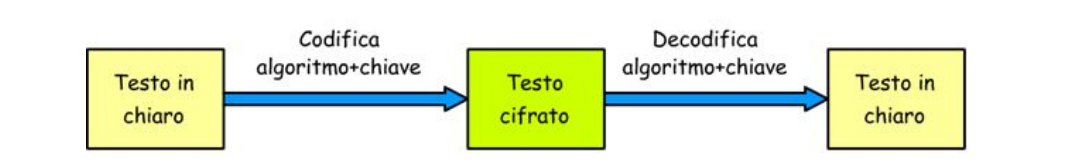
\includegraphics[width=\textwidth, keepaspectratio]{capitoli/crittografia/imgs/privata.png}
    \caption{Esempio del funzionamento della Crittografia Simmetrica.}
\end{figure}

La codifica e la decodifica sono eseguite dagli algoritmi crittografici assieme
ad una chiave che è la
stessa per entrambi i procedimenti. Tale chiave pertanto dovrà essere condivisa
tra le parti della
comunicazione. La segretezza, l'autenticazione e l'integrità dipendono dalla
segretezza della chiave.
Un sistema crittografico a chiave simmetrica molto conosciuto è il
\textbf{DES} ideato nel 1976 dalla IBM,
tuttora usato per cifrare files nei personal computer.
Questo sistema utilizza una chiave di 56 bit
(256 possibili chiavi).

\section{Crittografia a chiave Pubblica (asimmetrica)}

La crittografia asimmetrica, conosciuta anche come crittografia a coppia di chiavi,
crittografia a
chiave pubblica/privata o anche solo crittografia a chiave pubblica, è un tipo
di crittografia dove ad
ogni attore coinvolto nella comunicazione è associata una coppia di chiavi:

\begin{itemize}
    \item La chiave pubblica, che deve essere distribuita;
    \item La chiave privata, appunto personale e segreta;
\end{itemize}

Fra due interlocutori, non vi è dunque la necessità di scambiarsi le chiavi.
Se con una delle due
chiavi si cifra (codifica) un messaggio, allora quest'ultimo sarà decifrato solo
con l'altra.

\begin{figure}[H]
    \centering
    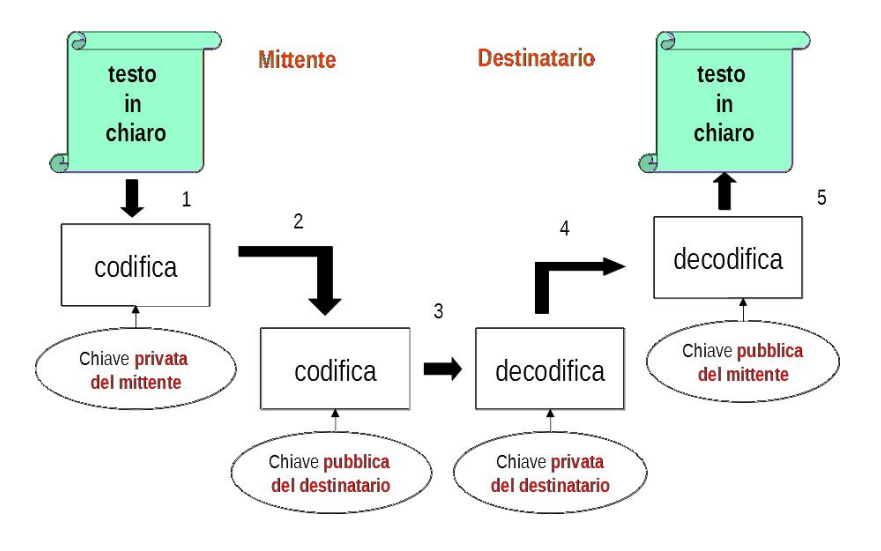
\includegraphics[width=\textwidth, keepaspectratio]{capitoli/crittografia/imgs/pubblica.png}
    \caption{Esempio del funzionamento della Crittografia Asimmetrica.}
\end{figure}

Gli attacchi a sistemi di crittografai sono detti attacchi
di \textbf{Crittoanalisi} e
come obbiettivo hanno quello di provare a dedurre la chiave che gli
permetterebbe di decriptare il testo.
I principali attacchi crittografici si basano sulle seguenti caratteristiche:

%%TODO: riscrivere a verso le varie descrizioni.
\begin{itemize}
    \item \textbf{CypherText only}: è noto solo il testo codificato;
    \item \textbf{Known plaintext}: il messaggio è cifrato ma il testo in chiaro è noto;
    \item \textbf{Chosen plaintext}: il testo in chiaro viene scelto in quale modo (per es. tutti 0, tutti 1, ecc);
    \item \textbf{Brute-force}: forza bruta, tentativi di attacco alla chiave finché non si trova quella giusta;
\end{itemize}

\paragraph{Crittografia Perfetta: } la crittografai si di dice Perfetta quando
nessun
testo codificato rilascia informazione alcuna né
sulla chiave usata per la codifica, né sul testo in chiaro,
il quale può essere recuperato se e solo se
la chiave è disponibile.
Si tratta di una situazione ideale, in quanto ogni tipo di crittoanalisi sarebbe
reso inutile e la
probabilità di ricavare informazioni supplementari da un testo codificato
sarebbe piuttosto nulla.
Purtroppo però, la crittografia in pratica non è quasi mai perfetta.

\section{Funzioni Hash}

Una funzione di hash è una funzione matematica che permette di ridurre una
qualunque stringa di
testo (indipendentemente dalla sua lunghezza) in una nuova stringa avente
precise caratteristiche
tra cui un numero di caratteri predefinito. A partire da un input X, in
altre parole, sarà possibile
generare un input Y che avrà delle caratteristiche ben definite.
A prescindere dal tipo di funzione di hashing tutte hanno dei punti in comune:

\begin{itemize}
    \item \textbf{Costanza}: a parità di input la stessa funzione di hash
          restituirà sempre la stessa stringa
          alfanumerica; ad ogni input, in altre parole, corrisponde sempre e
          inevitabilmente lo stesso
          output;
    \item \textbf{Irreversibilità}: mentre è sempre possibile riprodurre
          l'output conoscendo l'input originario
          col quale l'output è stato generato non è però possibile fare
          il percorso inverso, non si può
          quindi a partire da una stringa alfanumerica risalire al contenuto
          iniziale dell'input;
    \item \textbf{Determinismo}: indipendentemente da quanto sia lungo l'input,
          la funzione di hash restituirà
          sempre una stringa alfanumerica di un numero determinato di caratteri;
    \item \textbf{Effetto} valanga: non importa quanto l'input sia lungo e
          complesso, è sufficiente una
          variazione infinitesimale dell'input per generare un output
          completamente differente;
\end{itemize}

\section{Firma Digitale}

La firma digitale è una tecnologia con cui possono essere
effettivamente soddisfatti tutti i requisiti richiesti per dare validità
legale ad un documento elettronico firmato digitalmente;
garantisce i servizi di integrità, autenticazione e non ripudio.
Firmare non è esattamente codificare: firmare digitalmente un documento è spesso
utile perché evita di
codificare l'intero file in quanto ciò può richiedere un
tempo elevato. Verificare una firma, quindi, non significa
decodificare.

\begin{figure}[H]
    \centering
    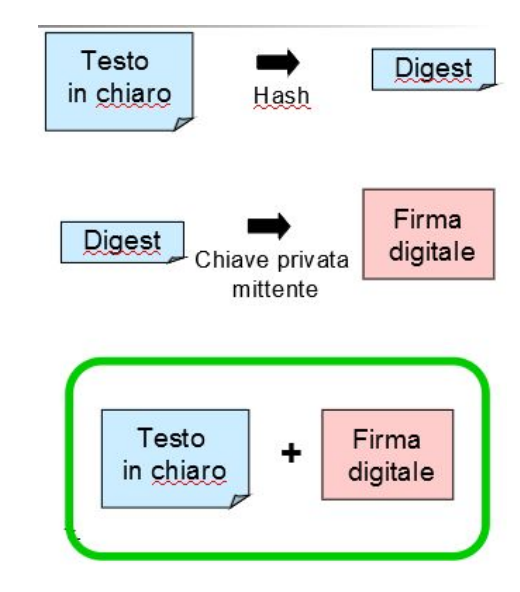
\includegraphics[width=\textwidth, keepaspectratio]{capitoli/crittografia/imgs/firmad.png}
\end{figure}

\subsection{Creazione della Firma}

La firma digitale viene realizzata tramite tecniche
crittografiche a
chiave pubblica insieme all'utilizzo di particolari
funzioni matematiche, chiamate funzioni hash
unidirezionali. Il processo di firma digitale passa
attraverso tre fasi:

\begin{enumerate}
    \item Generazione dell'impronta digitale.
    \item Generazione della firma.
    \item Apposizione della firma.
\end{enumerate}

Nella prima fase viene applicata al documento in
chiaro una funzione di hash appositamente
studiata che produce una stringa binaria di
lunghezza costante e piccola, normalmente 128 o 160
bit, chiamata “digest message”, ossia impronta
digitale.
Poiché la dimensione del digest message è fissa,
e molto più piccola di quella del messaggio
originale, la generazione della firma risulta
estremamente rapida. Utilizzare le funzioni hash
consente di evitare che per la generazione della
firma sia necessario applicare l'algoritmo di
cifratura all'intero testo che può essere molto lungo.
Mediante un software adatto si genera una coppia di
chiavi da utilizzare: una che verrà mantenuta
segreta per l'apposizione della firma; l'altra, destinata alla verifica, che
verrà resa pubblica. Quindi
la seconda fase, la generazione della firma, consiste semplicemente nella
cifratura con la propria
chiave privata dell'impronta digitale generata in precedenza.
Nell'ultima fase, la firma digitale generata precedentemente viene aggiunta in
una posizione
predefinita, normalmente alla fine del testo del documento.
E' da tenere presente che l'apposizione della firma digitale non garantisce la
confidenzialità del
testo, perché questo viene inviato in chiaro. Serve solo a garantirne integrità
e autenticità:

\begin{itemize}
    \item \textbf{Autenticità}: Il messaggio arriva proprio da chi dice di essere il mittente;
    \item \textbf{Integrità}: Il messaggio non ha subito modifiche o manomissioni;
\end{itemize}

\subsection{Verifica della Firma}

Il destinatario ottiene testo in chiaro con apposta la firma digitale.
Per comodità viene inviata anche la chiave pubblica del mittente. A
questo punto gli step sono:

\begin{enumerate}
    \item Separare il testo dalla firma;
    \item Decodificare la firma con la chiave pubblica del mittente;
    \item Calcolare il digest del testo tramite la funzione di hash;
    \item Verificare che i due digest coincidano. In caso positivo si ha
          la conferma del fatto che il documento è integro e non è stato
          sottoposto a modifiche.
\end{enumerate}

\section{Certificato Digitale}

Nella crittografia asimmetrica un \textbf{certificato digitale} è un
documento elettronico che attesta
l'associazione univoca tra una chiave pubblica e l'identità di un soggetto.
Il certificato digitale contiene informazioni sulla chiave,
sull'identità del proprietario
(denominato soggetto) e sulla firma digitale di un'entità che ha verificato
i contenuti del certificato
(denominato emittente) e riconosciuta come \textbf{CA}
(\textit{Certification Authority}).
Tale certificato, infatti, è
a sua volta autenticato per evitarne la falsificazione, sempre attraverso
firma digitale, ovvero viene
cifrato con la chiave privata dell'associazione, la quale fornisce poi la
rispettiva chiave pubblica per
verificarlo.
Ad una CA sono assegnati 10 compiti:
\begin{enumerate}
    \item Identificare con certezza la persona che fa richiesta della certificazione della chiave
          pubblica;
    \item Rilasciare e rendere pubblico il certificato;
    \item Garantire l'accesso telematico al registro delle chiavi pubbliche;
    \item Informare i richiedenti sulla procedura di certificazione;
    \item Dichiarare la propria politica di sicurezza;
    \item Attenersi alle norme sul trattamento di dati personali;
    \item Non rendersi depositario delle chiavi private;
    \item Procedere alla revoca o alla sospensione dei certificati in caso di richiesta dell'interessato o
          venendo a conoscenza di abusi o falsificazioni, ecc;
    \item Rendere pubblica la revoca o la sospensione delle chiavi;
    \item Assicurare la corretta manutenzione del sistema di certificazione.
\end{enumerate}

\subsection{Formato x.509}

Il formato più comune per i certificati di chiave pubblica è definito da X.509, raccomandato dalla
ITU (International Telecommunication Union).
Il certificato viene firmato da chi lo emette. “Codice identificativo
dell’emittente” è univoco per ogni
CA esistente. La firma garantisce il fatto che il documento è autentico,
cioè che è stato scritto dal
“nome soggetto” e che è stato verificato da “ente emettitore”.
E’ importante specificare il “periodo di validità” poiché la stessa firma
(e la coppia chiave
pubblica-privata) ha una validità temporale. Se questa dovesse scadere,
il certificato va riemesso.
Ciò viene fatto anche nel momento in cui i ruoli (specificati nel campo
“estensioni”) di chi partecipa
alla sottoscrizione cambiano.
Viene anche specificato l’elenco degli algoritmi utilizzati per
l’apposizione della firma con i relativi
parametri.

% TODO valutare se inserire immagine

\subsection{Ottenere un certificato Digitale}

Sono richieste le seguenti fasi: l’utente genera sul proprio PC una coppia
di chiavi. I browser
comuni offrono tale il servizio; la chiave privata è memorizzata localmente
in un file nascosto. Per
avere una maggiore sicurezza si potrebbero memorizzare le chiavi su una
SmartCard protetta da
un PIN. L’utente invia alla CA una richiesta di certificato, insieme alla
chiave pubblica generata; la
CA autentica il richiedente, di solito chiedendogli di recarsi di persona
ad uno sportello di \textbf{LVP}
(\textit{Local Validation Point}) collegato con la CA.
A questo punto, verificata l’identità, la CA emette il certificato,
lo invia al richiedente tramite posta
elettronica ed inserisce la chiave certificata nel registro delle chiavi
pubbliche.
L’intera procedura sopra descritta accade nell’ambito di una \textbf{PKI}
(\textit{Public Key Infrastructure}), la cui
struttura minima prevede la presenza di una CA ed un LVP; in generale
sono ammessi più LVP.
Una PKI può avere una struttura gerarchica in cui alcune CA certificano
altre CA, ottenendo una
“catena di fiducia”. Secondo tale struttura: la “Root CA” certifica le
CA di primo livello; le CA di
primo livello certificano le CA di secondo livello; le CA di ultimo
livello certificano il singolo utente.

\subsection{Revoca del certificato}

Il certificato può essere revocato per varie ragioni: cambio dei dati
personali (email, recapito, ecc),
licenziamento, dimissioni, Compromissione della chiave privata, ecc.
Può avvenire anche su richiesta da parte dell’utente o dell’emettitore.

\subsection{Certificate Revocation List}

Un \textbf{CRL} è un elenco di certificati digitali che sono stati revocati
dalla CA,
prima della data di scadenza pianificata e non dovrebbero più essere
considerati attendibili.
Viene generato e pubblicato periodicamente, spesso ad un intervallo di
tempo definito. Ad ogni
pubblicazione, infatti, viene anche comunicata la data del successivo
aggiornamento.
Viene rilasciato da un'entità autorizzata che è tipicamente la CA
che ha anche rilasciato i certificati
corrispondenti.
%TODO cercare immagine migliore

\begin{figure}[H]
    \centering
    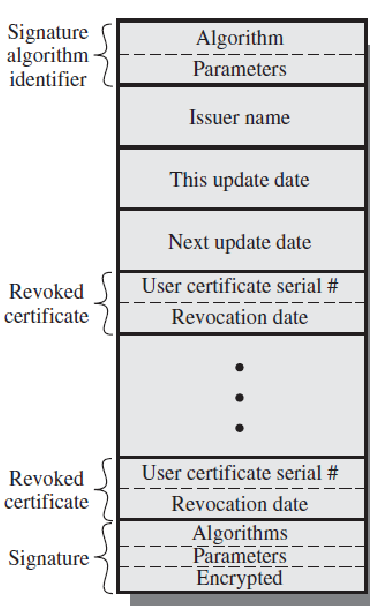
\includegraphics[width=10cm, keepaspectratio]{capitoli/crittografia/imgs/CRL.png}
\end{figure}

\section{Protocolli di Sicurezza}

Un protocollo di sicurezza è una sequenza di azioni (passi) che
coinvolge due o più parti,
finalizzata all’instaurazione di una comunicazione sicura tra di esse,
al sicuro dalle azioni di un
possibile intruso. L’insieme dei passi specificati costituisce la sessione
del protocollo.
Servono per garantire l’autenticità dell’utente.

\paragraph{Nonce: }
In crittografia il termine nonce indica un numero, generalmente casuale
o pseudo-casuale,
che ha un utilizzo unico. Nonce deriva infatti dall'espressione inglese
“for the nonce”, che significa
appunto "per l'occasione". Un nonce viene utilizzato spesso nei protocolli
di autenticazione per
assicurare che i dati scambiati nelle vecchie comunicazioni non possano
essere utilizzati in
attacchi di tipo replay attack.\\

%TODO da capire meglio il DY
In ogni protocollo viene utilizzata una \textbf{spia DY}, la quale possiede una serie di capacità che le
permettono di individuare l’intruder:
\begin{itemize}
    \item Intercettare messaggi e prevenirne il recapito;
    \item Far rimbalzare a piacere i messaggi intercettati;
    \item Imparare i testi in chiaro e i testi codificati;
    \item Tentare di decriptare con tutte le chiavi note;
    \item Utilizzare le proprie credenziali legali;
    \item Ottenere certe credenziali illegalmente;
    \item Creare messaggi fasulli da componenti già note;
\end{itemize}

% TODO Cambiare nomenclatura robe con aspetto matematico
\section{Autenticazione di utenti remoti con Needham-Schr\"{o}der (1978)}

Sono stati definiti vari protocolli a riguardo. L’obiettivo è quello di
garantire l’autenticazione
dell’utente da remoto appunto, ottenuta dallo scambio segreto dei nonce.
Needham-Schröder è basato sulla crittografia asimmetrica e permette
di assicurare la mutua
autenticazione tra due entità di rete. Nella sua forma proposta
non è sicuro.
Utilizzeremo dei messaggi fatti così:

\begin{itemize}
    \item Nomi di utenti: A, B, C…
    \item Chiavi crittografiche
          \begin{itemize}
              \item a lungo termine: Ka, Kb…
              \item a breve termine: Kab… (chiavi di sessione)
          \end{itemize}
    \item Nonce: Na, Nb…
    \item Timestamp: Ta, Tb…
    \item Digest
    \item Label: “trasferisci denaro”, “collegati alla porta xy”…
\end{itemize}

I messaggi base possono essere a loro volta composti:
\begin{itemize}
    \item Concatenati: m,m’…
    \item Criptati: mK, {m,m’}K…
\end{itemize}

Il protocollo presuppone una PKI (infrastruttura a chiave pubblica)
con crittografia perfetta.

\begin{figure}[H]
    \centering
    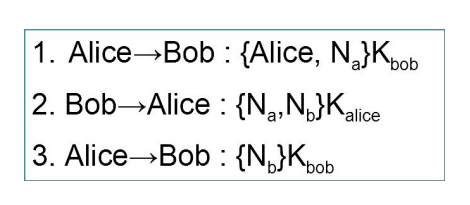
\includegraphics[width=\textwidth, keepaspectratio]{capitoli/crittografia/imgs/alieno.png}
\end{figure}

Alice vuole identificarsi con Bob, quindi Bob alla fine dell’applicazione del protocollo dovrà essere
sicuro di aver comunicato con Alice.
\begin{enumerate}
    \item Alice invia un messaggio criptato con la
          chiave pubblica di Bob, che quindi solo lui potrà
          aprire. Il nonce Na permette di capire se il
          messaggio che è stato inviato è nuovo. Si
          analizzano tutte i nonce già utilizzate per
          verificare che essa sia appunto un valore mai
          visto;
    \item Bob riceve il messaggio e lo apre. Una volta
          letto, risponde ad Alice: invia indietro il nonce
          Na ricevuta più uno nuovo, Nb, questa volta
          per fare in modo che sia lui ad autenticarsi con
          Alice. Il messaggio è codificato con la K
          pubblica di Alice;
    \item Alice riceve la risposta e invia a sua volta
          Nb a Bob. A questo punto Bob è sicuro di poter
          parlare con Alice.
\end{enumerate}

L’autenticazione è garantita dal fatto che i nonce non
possono necessariamente avere lo stesso
numero e che le chiavi a lungo termine non possono
essere compromesse.
La prova del fatto che il messaggio 1 sia stato inviato
da Alice ci viene data dalla chiave \(K_{alice}\) nel
messaggio 2 e quindi sappiamo che solo lei lo può aprire.

%TODO Mettere alieno
\subsection{Attacco di Lowe (1995)}

Uno studente di Cambridge, Lowe, dimostra che il protocollo appena visto non funziona perché è
possibile attaccarlo. Ciò significa che qualcun altro potrebbe riuscire a spacciarsi per Alice con Bob
(in riferimento all’esempio precedente).

\paragraph{Nel Dettaglio: }
Ive è uno dei partecipanti al protocollo:

\begin{enumerate}
    \item[1.]  Alice vuole comunicare con lei. Ive (che però è l’intruder)
        apre il messaggio inviato da Alice
        (grazie alla sua chiave privata) e lo invia a Bob;
    \item[1'.] Ive, che vuole spacciarsi per Alice nei confronti di Bob,
        ricodifica il messaggio prima di inoltrarlo
        a Bob;
    \item[2'.] Bob segue le regole del protocollo N-S ed invia ad Alice
            {Na, Nb} criptato con Kalice. Ive
        potrebbe lasciare andare il messaggio oppure
    \item[2.] potrebbe intercettarlo e rispedirlo ad Alice.
\end{enumerate}
Tutti i partecipanti, nel momento in cui ricevono dei messaggi, devono
verificare che gli invii
corrispondano a quanto specificato nel protocollo.Se così non fosse, tutta
l’esecuzione cadrebbe e
verrebbe riavviata da zero.

\begin{enumerate}
    \item[2.] Il messaggio inviato da Ive ad Alice ha come primo
        elemento Na (il nonce di Alice), e come secondo elemento Nb
        (il nonce di Bob) che Alice crede sia stato
        generato da Ive;
    \item[3.] Alice inoltra Nb ad Ive criptando con la K di Ive;
    \item[3'.] Ive apre il messaggio e lo invia a Bob, criptato con Kbob
\end{enumerate}

Bob, che è l’utente di cui il protocollo si approfitta, riceve Nb.
Controlla che il nonce sia quella che
ha effettivamente inventato e a quel punto è sicuro di parlare con Alice.
Ive ha quindi usato il nonce che ha inventato Alice per approfittarsi di
Bob. Ha effettuato un
\textit{attacco di autenticazione}, in quanto Bob pensa di comunicare con
Alice, ma in realtà sta parlando
con Ive.
Ive si spaccerà per Alice con Bob visto che si è autenticata al suo posto,
quindi può chiedergli dei
servizi. Per esempio, se Bob rappresentasse una banca, Ive potrebbe
richiedere un trasferimento
di denaro dal conto di Alice al proprio.
Lo stesso tipo di attacco può essere studiato nella tassonomia BUG. Tale
soluzione è deprecata
ma continua ad essere utilizzata.
Sappiamo che Alice ha condiviso con Ive il nonce Na da lei generata, ma
questa in realtà è stata
inoltrata anche a Bob. Bob, nel caso in cui avesse delle intenzioni
malevole, potrebbe utilizzare Na
ai danni di Alice: se Alice vedesse arrivare un messaggio contenente Na
e Nb, infatti, penserebbe
che questo sia stato inviato da Ive. Bob però, conoscendo l’importanza di
Na, potrebbe agire,
stavolta vendicandosi su Ive.
Il protocollo presenta delle vulnerabilità, quindi non è del tutto sicuro.
Per ovviare a questo
problema, si potrebbe aggiungere una comunicazione fuori banda. Ogni qual
volta un utente voglia
autenticarsi, prima di eseguire una sua qualunque istruzione, è necessario
verificarne l’effettiva
identità.

\section{Protocollo di sicurezza di Woo-Lam (anni 80)}

Usa la crittografia simmetrica e usa un TTP (Trusted Third Party), che
possiede un database di
tutte le chiavi. Un TTP è un'entità che facilita le interazioni tra due
parti che si fidano entrambe
della “terza parte”.
L'obiettivo del protocollo è che Alice (A) riesca ad autenticarsi
con Bob (B).

\begin{figure}[H]
    \centering
    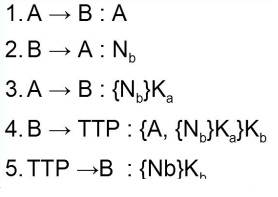
\includegraphics[width=10cm, keepaspectratio]{capitoli/crittografia/imgs/Mulan.png}
\end{figure}

\begin{enumerate}
    \item A invia un messaggio pubblico a B;
    \item B invia ad A una nonce Nb ad A per verificare che stia
          effettivamente comunicando con lei. Anche questo messaggio è
          pubblico;
    \item A riceve Nb e la inoltra di risposta a Bob, ma criptata con
          Ka. Ka è una chiave simmetrica che ha in condivisione con il
          TTP e che B non può aprire. Bob deve verificare che Ka
          appartenga davvero ad A;
    \item B invia la richiesta al TTP di aprire il messaggio per verificare
          l’appartenenza di Ka. Il
          messaggio è criptato con Kb e lo può aprire solo il TTP poiché condivide
          le chiavi
          simmetriche con B;
    \item Il TTP, una volta decifrato il messaggio e ottenuto Nb, lo inoltra a B.
          B apre il messaggio
          finale perché possiede Kb e verifica che Nb sia la nonce che ha inviato ad A.
          Se è così,
          significa che B ha effettivamente comunicato con A. La decodifica di {Nb}Ka
          funziona solo se Ka appartiene ad A.
\end{enumerate}

\subsection{Attacco su Woo-Lam}

Anche detto “interlacciamento di sessioni”.
\begin{figure}[H]
    \centering
    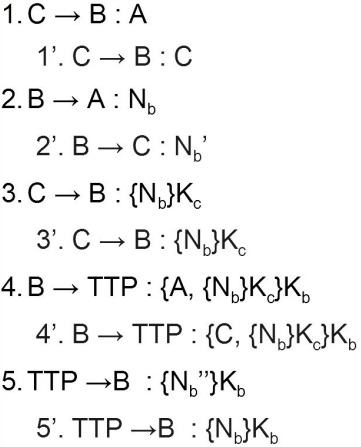
\includegraphics[width=8cm, keepaspectratio]{capitoli/crittografia/imgs/mulan2.png}
\end{figure}
\begin{enumerate}
    \item[1.] C è l’attaccante che si vuole spacciare per A con
        B e invia un messaggio a B confermando ciò;
    \item[1'.] C invia anche un altro messaggio a B dove
        afferma invece di essere C; Alla ricezione dei due
        messaggi, B segue il protocollo e genera due nonce;
    \item[2.] In risposta ad A genera Nb;
    \item[2'.] In risposta a C genera Nb’;
        C intercetta i messaggi e quindi anche le due nonce.
    \item[3/3'.] C invia Nb criptata con Kc a B due volte;
        B quindi riceve lo stesso messaggio due volte.
    \item[4.] Supponendo che un messaggio sia stato inviato
        da A, B invia al TTP la nonce Nb che ha ricevuto. Il
        messaggio è poi criptato con Kb;
    \item[4'.] B invia un altro messaggio al TTP ma questa
        volta con C all’interno.
    \item[5.] TTP invia a B la nonce Nb’’ ottenuta a partire dalla
        decifratura del messaggio 4 (nonce completamente
        sbagliata);
    \item[5'.] TTP invia a B la nonce Nb’ ottenuta a partire dalla
        decifratura del messaggio 4
\end{enumerate}

B si renderà conto del fatto che Nb’ è stata inviata da A. Quindi B ha
autenticato C al posto di A,
Infatti, il messaggio di autenticazione che avrebbe dovuto prendere in
considerazione era il 4 con
nonce Nb’’.
Se B attiva due comunicazioni contemporaneamente, non può sapere in che
ordine arriveranno i
messaggi.
Il protocollo sembrerebbe funzionare ma in realtà non è così.
Si porta all'attenzione dell'egregio lettore che esiste anche la versione
simmetrica di Needham-Schröder (questa è un informazione dalla
dubbia utilità).


